%%%%% Document Setup %%%%%%%%

\documentclass[12pt, onecolumn, nofootinbib]{revtex4}    % Font size (12pt) and column number (one or two).

\usepackage{times}                          % Times New Roman font type
\usepackage[dvipsnames]{xcolor}
\usepackage[a4paper, left=2.5cm, right=2.5cm,
 top=2.5cm, bottom=2.5cm]{geometry}       % Defines paper size and margin length
%\usepackage{url}
\usepackage{tikz}
\renewcommand{\baselinestretch}{1.15}     % Defines the line spacing
\usepackage{hyperref}
\hypersetup{pdfborder={0 0 0}}
\usepackage{pagecolor}
\pagecolor{white}
\usepackage[font=small,
labelfont=bf]{caption}                      % Defines caption font size and caption title bolded

\usepackage{graphics,graphicx,epsfig,ulem}	% Makes sure all graphics works
\usepackage{amsmath} 						% Adds mathematical features for equations

\usepackage{etoolbox}                       % Customise date to preferred format
\makeatletter
\patchcmd{\frontmatter@RRAP@format}{(}{}{}{}
\patchcmd{\frontmatter@RRAP@format}{)}{}{}{}
\renewcommand\Dated@name{}
\makeatother

\usepackage{fancyhdr}
\usepackage{ amssymb }

\pagestyle{fancy}                           % Insert header
\renewcommand{\headrulewidth}{0pt}
\lhead{\small Georgia Hills}                          % Your name
\rhead{\small Strong Coupling Constant Extraction at energy s = ${\sqrt{13}}$ TeV}            % Your report title               

\def\thesection{\arabic{section}}

\def\bibsection{\section*{References}}        % Position reference section correctly


%%%%% Document %%%%%
\begin{document}                     


\title{Strong Coupling Constant Extraction} 
\date{Submitted: \today{}}
\author{Georgia Hills}
\affiliation{\normalfont Level 4 Project, MPhys Natural Sciences\\ Supervisor: Dr D. Ma\^itre\\ Department of Physics, Durham University}

\begin{abstract}              
 The aim of this report is to extract a value of the strong coupling constant ${\alpha_s}$. The extraction is presented at Next-to-Leading Order. Factorisation and Renormalisation scales, and the practical implications this had during the extraction, are included. A ${\chi^2}$  fit was performed in order to extract ${\alpha_s}$. Covariance matrices are calculated using predictions generated from PDF'S, and experimental ${Z}$+ 2,3,4 jets data generated by ATLAS at CERN.  The value obtained is ${\alpha_s(M_Z) = **** \pm ^{//}_{//}}$.


\end{abstract}


\maketitle


\tableofcontents
%\let\toc@pre\relax
%\let\toc@post\relax

\newpage


\section{Introduction} \label{intro}

The strong coupling constant, ${\alpha_s}$ is a parameter of Quantum Chromodynamics (QCD) and QCD describes the strong interaction \cite{DMP}.  The constant is a parameter of the standard model, so in order for further predictions to be made accurate and well-known values of its parameters is required. The strong interaction is only experienced by particles with colour charge; quarks and gluons \cite{PPB}. ${\alpha_s}$ indicates the strength of this interaction. The strong force is responsible for ordinary matter being stable. It binds quarks together to form protons and neutrons and then binds nucleons together to form nuclei. ${\alpha_s}$ cannot be predicted from first principles, so must be extracted from experiments.  The data for extracting ${\alpha _s}$ is collected by the ATLAS group at CERN and considers the cross-section of a collision event of two protons \cite{HEPD}. For simplicity the collision considered at tree level (no momenta loops) is known as the Drell-Yan process, where-in a quark of one proton and an anti-quark of another proton annihilate \cite{BOOK}. This is summarised as: \begin{equation} \label{DRELL} pp \xrightarrow{Z/\gamma}  l^+l^- + X, \end{equation} where ${X}$ can be a number of things, and the ${Z}$ boson and the photon, ${\gamma}$, are the propagators. In the lowest energy process just the lepton pair ${(l^+l^-)}$ is created. However protons are hadrons which are composed of partons, namely quarks and gluons. The partons inside the protons  interact and not the composite protons. Partons undergo inelastic collisions so the centre of mass energy of quarks and gluons is not fixed \footnote{The centre of mass energy is only defined statistically through Parton Distribution Functions (PDF) see section (\ref{PDF})}, thus a huge spectrum of energies can be considered.  The partons are charged under the strong force and they emit vast amounts of collinear radiation which gives rise to jets, shown as ${X}$ in equation (\ref{DRELL}) \cite{PHD}. Jets are a collimated spray of hadrons.These jets are  created from energetic quarks or gluons that decay into hadrons. Jets of ${Z}$ boson + 2,3,4 differential cross section are used to extract ${\alpha _s}$ \cite{HEPP}. The cross-section data is taken at a centre of mass  energy of ${s = \sqrt{13}}$ TeV for multiple jet processes \cite{HEPP}. Previous values of ${\alpha _s}$ have been extracted using similar methods and yielded a value of ${\alpha _s(M_z) = 0.1178^{+0.0051}_{-0.0043}}$ at a centre of mass energy of ${s=\sqrt{7}}$  TeV, where ${M_Z}$ is the mass of the ${Z}$ boson. The world average is given as ${\alpha _s(M_z) = 0.1181 \pm 0.0011}$ \cite{PPB}. 

\section{The Expansion of ${\bold{\alpha_s}}$}

The strong coupling constant ${\alpha_s}$ can be expanded perturbatively to different orders for high energy scales. The value of ${\alpha _s}$ presented here is at next-to-leading order (NLO).  For this extraction NLO specifically means for a number of jets $j$, the observable, ${\mathcal{O}}$, depends on ${\alpha _s}$ as: \begin{equation} \label{expan} \mathcal{O} \propto \alpha _s^j (1 + C\times\alpha_s), \end{equation} where ${C}$ is a correction constant. This equation is derived using the fact that the cross section of each strong interaction in a Feynman diagram is proportional to ${\alpha_s}$ term. Hence the number of jets signifies the number of strong interactions. From equation (\ref{expan}) the different number of jets results in different sensitivities.  A larger number of jets corresponds to a higher theoretical and experimental uncertainty. This is because a higher energy is required for larger number of jets so they are less likely to occur, thus less data, and hence a larger uncertainty. A higher number of jets is also more difficult to simulate in Monte-Carlo simulations, see section (\ref{PDF}). However as the jet number increases so does the order of ${\alpha_s}$ according to equation (\ref{expan}), which means there is an increase in sensitivity. Thus the increased uncertainty is somewhat compensated for. Hence the degrees of precision for each number of jets can be compared so the best method for extraction is to combine the 3 multiplicities to find a final value of ${\alpha _s}$ \cite{DMP}. 
\begin{figure} 
	\begin{center}
		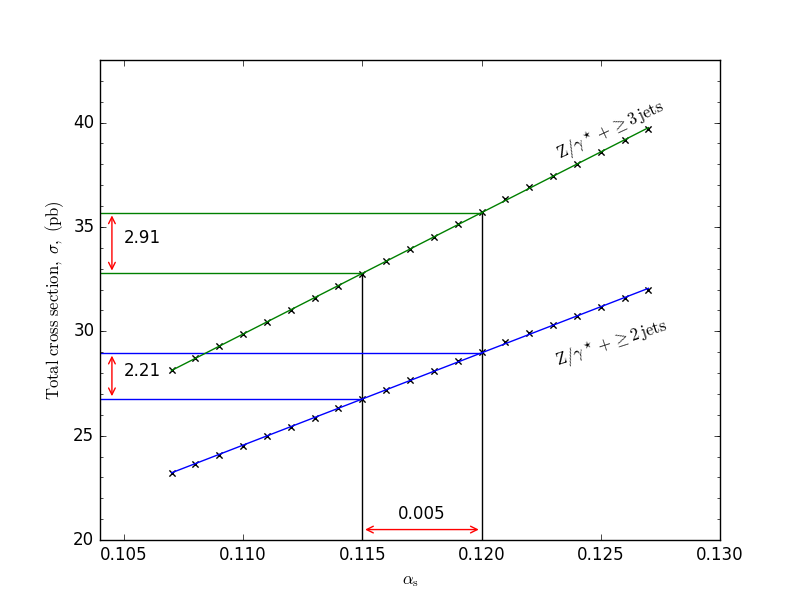
\includegraphics[width=1 \textwidth]{2jetvs3jet_totxsection.png}
		\caption{The variation of the error of cross section covered for a given range of ${\alpha_s}$. A higher number of jets corresponds to a larger cross section considered hence a lower error on that cross section measurement. The PDF used was MSTW08cl for the central scale. }
		\label{2jetvs3jet
		}
	\end{center}
\end{figure}

\subsection{Previous Extraction Methods}
Previously a similar method for extracting ${\alpha_s}$ was used at a centre of mass energy ${s = \sqrt{7}}$ TeV, compared to this extraction at ${s = \sqrt{13}}$ TeV. The advantage of the increase in ${s}$ is such that it increases the number of scattering events which generates more data also. At higher energies, it is more likely that more jets are produced for a fixed jet energy, so more data can be obtained at these higher multiplicities. This reduces the experimental uncertainty and thus the overall uncertainty in the extraction of ${\alpha_s}$. 

There are many different methods for extracting ${\alpha_s}$, each with different short-comings and benefits. Previous methods have extracted ${\alpha_s}$ by comparing experimental data from deep inelastic scattering,  hadronic ${\tau}$ decays, against predictions from the theory,  and hadronic experiments, see \cite{PPB} for an overview. Extractions based on the \textit{R} ratio are of order ${(\alpha_s)^0}$. Expansion of observables which depend on ${\alpha_s}$ start at next-to leading order, ${(\alpha_s)^1}$, and use data from 3-jet rates and event shapes at ${e^+e^-}$. At hadron colliders the ratio of three to two jet production \cite{2to3} and the transfer energy-energy correlation \cite{en2en} starts at order ${(\alpha_s)^1}$ also. To start expansion at ${(\alpha_s)^2}$ inclusive jet cross sections are used \cite{inc}. The observables with the highest sensitivity used so far, whose expansion starts at order ${(\alpha_s)^3}$ are  the five-jet production rates at LEP \cite{LEP}, the heavy quarkonia hadronic decay width \cite{HAD} and the 3-jet inclusive observables \cite{3jet}. The previous extraction, similair to this one peformed at ${s=\sqrt{7}}$ TeV was of order ${(\alpha_s})^4$ \cite{DMP}.These methods have different levels of sensitivity which depends on where the expansion of ${\alpha_s}$ starts. It is usually the case that observables with a lower sensitivity to ${\alpha_s}$ can be measured more precisely than those with a higher sensitivity. \cite{DMP}. A visual comparison of different experimental techniques and their data is given in figure (\ref{allas}). 

\section{Theoretical Context and Motivation} 
The strong force is unique from the other Standard Model forces as it is described by an additional quantum number namely colour, of which there are three values. The need for colour charge can be explained by considering the ${\Delta^{++}}$ baryon which consists of three up quarks (uuu). As the baryon is formed of three identical fermions the overall wave-function needs to be anti-symmetric under exchange of two fermions, according to the Pauli Exclusion Principle. However the spin, parity and spatial parts of the wave-function are all symmetric under exchange of two fermions (as they are identical fermions), thus an additional anti-symmetric quantum number is needed, which we denote as colour charge \cite{BOOK}.
\subsection{The Context of QCD within the Standard Model.}

The Standard Model (SM) is well-tested and one of the most predictive theories in the history of physics. However it is not complete as it fails to explain the existence of dark matter and dark energy. This is why accurate measurements of constants is  key as in order to determine any discrepancies from the SM an accurate and well established knowledge of fundamental constants is required \cite{PHD}. The SM is given by ${SU(3)\times SU(2) \times U(1)}$. The ${SU(2) \times U(1)}$ part corresponds to the electroweak sector. The weak sector is mediated by the ${W^\pm}$ and ${Z}$ boson and gives rise to radioactive decay. Quantum electrodynamics gives rise to electromagnetism whose field is mediated by photons ${\mathcal{A}^\mu}$ \cite{PHD}. QCD is described by ${SU(3)}$ which gives rise to the strong force mediated by gluons \cite{PPB}. The special unitary \footnote{A unitary matrix is a matrix whose hermitian conjugate is the same as its' inverse} group ${SU(3)}$  means that the representation of the group consists of unitary 3x3 matrices with determinant 1 \cite{GROUP}.  SU(3) is a group that is non-abelian \footnote{Non-Abelian means that the group is Non-commutative.} and describes QCD which is a gauge \footnote{Gauge simply means that symmetries are defined locally.} field theory \cite{BOOK}. 

A coupling constant determines how strong an interaction between two particles is when compared to the kinetic term, which is the first term of the Lagrangian: \begin{equation} \label{Lag} \mathcal{L} = \sum_ {q} \overline{\psi}_{q,a} (i\gamma^\mu \partial_\mu \delta_{ab} - g_s \gamma^\mu t_{ab}^C \mathcal{A}_\mu^C  - m_q\delta_{ab})\psi_{q,b} - \frac{1}{4} F_{\mu\nu}^A F^{A \mu\nu}, \end{equation} where the Einstein Summation Convention has been used. The colour-indices, $a,b$, run from 1 to  ${N_c = 3}$, ${m_q}$ represents the mass of the quarks and ${q}$ represents the quark flavour of the spinor $\psi_{q,a}$. Quarks are the fundamental representation i.e. an irreducible representation, of the ${SU(3)}$ group, and the interaction between a quark and anti-quark is given by the first term of equation (\ref{Lag}). The QCD coupling constant is given the symbol ${g_s}$, which relates to ${\alpha_s}$ via: ${\alpha_s = \frac{g_s^2}{4\pi}.}$ The ${t_{ab}^C}$ are the generators of the SU(3) group and are eight 3x3 matrices. The field tensor ${F_{\mu\nu}^A}$, describes how the gluon field propagates, and is defined: \begin{equation}F_{\mu\nu}^A  = \partial_\mu \mathcal{A}_\nu^A  - \partial_\nu \mathcal{A}_\mu^A - g_s f^{ABC} \mathcal{A}_\mu^B \mathcal{A}_\nu^C  \qquad [t^A,t^B] = if^{ABC}t^C,  \end{equation} where ${f^{ABC}}$ are the structure constants of the ${SU(3)}$ group, analogous to the Levi-Civita symbol for ${SU(2)}$ \cite{PPB}. T The ${- g_s f^{ABC} \mathcal{A}_\mu^B \mathcal{A}_\nu^C}$ term describes how gluons, ${A_\mu^C}$, interact with themselves. This happens as gluons carry colour charge, unlike photons which do not carry electric charge. ${C}$ runs from 1 to ${N_C^2 -1 = 8}$, implying that there are 8 types of gluon, which are massless. 

\subsection{Asymptotic Freedom and Colour Confinement} \label{colour}

 When a quark and gluon interact, represented by the second term in equation (\ref{Lag}) the quark's colour is "rotated" in ${SU(3)}$ colour space, analogous to an object rotating in physical space, and it's rotation being described by a rotation matrix. Consider rotating a circle in a 2D plane no matter how far we rotate the circle about its centre, the result is the same as the beginning. Analogously when rotating an observable in colour space it must be colour neutral for the observable to be symmetric under that ${SU(3)}$ rotation. Indeed experimentally we find this always to be true and this gauge symmetry is never broken. All observed objects are colour neutral and quarks and gluons which carry colour charge are never directly observed. This is known as colour confinement \cite{BOOK}. If we tried to separate quarks or gluons inside a colour neutral object, their separation is at a measurable scale when the potential energy of their separation is so large that is greatly surpasses the energy needed to create new particles. Particles being confined implies that ${\alpha_s}$ is large \footnote{ ${\alpha _s}$ is said to be strong at this energy scale as it is of higher magnitude than the electric charge.} when their separation is large where the energy is small. For low energy scales ${\alpha_s}$ is large, so perturbation theory cannot be used.  
 
However quarks and gluons directly interact at high energies implying that ${\alpha_s}$ is small here, so perturbation theory is valid. This is known as asymptotic freedom. Hence the strong coupling constant ${\alpha _s}$ is not constant and varies at different energy scales, thus we re-name it the running coupling constant \cite{BOOK}, its behaviour with energy is shown in fig (\ref{allas}). 
\begin{figure} 
	\begin{center}
		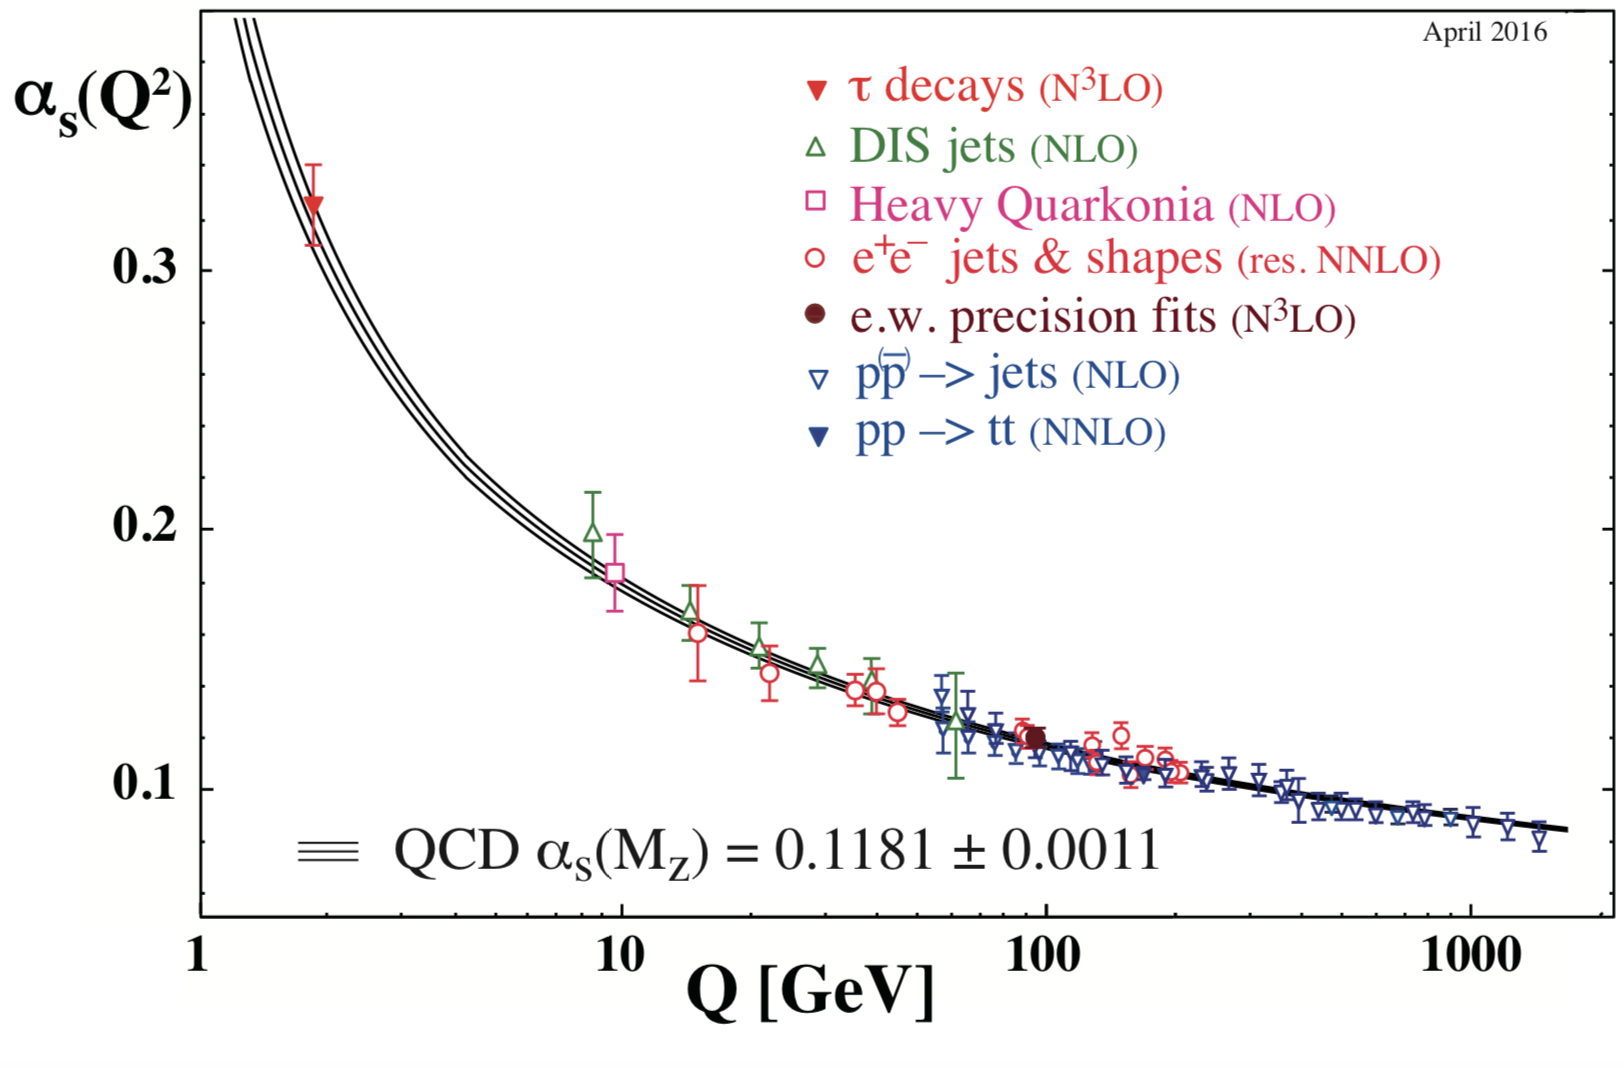
\includegraphics[width=1 \textwidth]{as_allq.jpg}
		\caption{Summary of measurements of ${\alpha_s}$ as a function of ${Q}$ the energy scale. The degree of QCD perturbation theory is given in brackets (NLO: next-to-leading order), etc. This graph was produced by the \textit{Particle Data Group}, see \cite{PPB}}
		\label{allas}
	\end{center}
\end{figure}


\section{Experimental Set-up at the LHC} \label{EXP}
\begin{figure}
	\minipage{0.5\textwidth}
		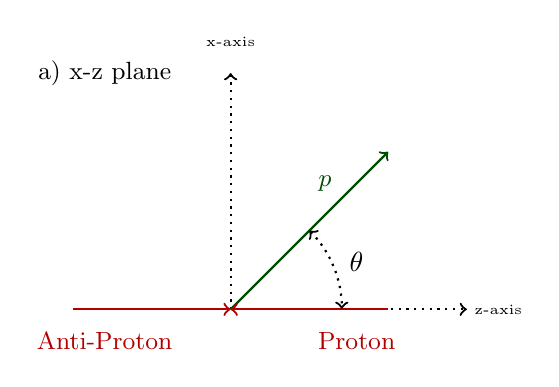
\begin{tikzpicture}[scale=2]
			\draw[dotted, ->, thick] (0,0) --(0,1.5);
			\draw[dotted, ->, thick] (-1,0) --(1.5,0);
			\draw[->, green!30!black, thick] (0,0) --(1,1);
			\draw[->, black!30!red, thick] (-1,0) --(0,0); 
			\draw[<-, black!30!red, thick] (0,0) --(1,0);
			\draw[dotted, <->, thick] (0.5,0.5) arc [start angle= 45, end angle=0, radius = 20pt ];
			\draw (0.8,0.3) node {$\theta$};
			\draw[green!30!black] (0.6,0.8) node {\small $p$};
			\draw[black!30!red] (-0.8, -0.2) node {\small Anti-Proton};
			\draw[black!30!red] (0.8,-0.2) node {\small Proton};
			\draw (0,1.7) node {\tiny x-axis};
			\draw (1.7,0) node {\tiny z-axis};
			\draw (-0.8,1.5) node {\small a) x-z plane};
		\end{tikzpicture}
	\endminipage\hfill
	\minipage{0.5\textwidth}
		\begin{tikzpicture}[scale=2]
			\draw[dotted, ->, thick] (0,0) --(0,1.5);
			\draw[dotted, ->, thick] (0,0) --(1.5,0);
			\draw[->, blue, thick] (0,0) --(1,1);
			\draw[dotted, <->, thick] (0.5,0.5) arc [start angle= 45, end angle=0, radius = 20pt ];
			\draw (0.8, 0.3) node {$\phi$};
			\draw[blue] (0.6,0.8) node {\small $p_T$};
			\draw[black!30!red, fill=black!30!red] (0,0) circle (.2ex);
			\draw (0,1.7) node {\tiny x-axis};
			\draw (1.7,0) node {\tiny y-axis};
			\draw (-0.8,1.6) node {\small b) ``Transverse''};
			\draw (-0.8,1.4) node {\small x-y plane};
		\end{tikzpicture}
	\endminipage
	\caption{a) The scattering centre of two protons, given by the red arrows, with centre of mass scattering angle ${\theta}$ and momentum ${p}$ of the products. b) ${\phi}$ is the azimuthal scattering angle, ${p_T}$ is the transverse momentum which is given by ${p_T = p\sin{\theta}}$ \cite{Sca}.}
	\label{SCAT}
\end{figure}


Firstly, figure (\ref{SCAT}) shows the physical scattering set up, and how angles are defined. A useful quantity to now define is the rapidity, ${\eta = -\ln[\frac{\tan{\theta}}{2}]}$. We cannot measure the momentum fraction carried by the interacting quarks within the proton and anti-proton, so you cannot know the frame in which the collision occurred but the rapidity is lorentz invariant so it does not matter in which frame it is evaluated, hence its information is decoupled from the frame.  This allows us to define a useful co-ordinate system, ``${\eta-\phi}$'' space, where-in the direction of an outgoing jet is represented by a point in ${\eta-\phi}$ space. 

\subsection{Jet Algorithms}
It is useful to discuss how jets are quantified and how they are measured. As discussed in section (\ref{intro}) strongly interacting particles experience significant final state radiation. This is further amplified by the size of the strong coupling constant, which is an order of magnitude larger than the electromagnetic ones in the energy regime below the colour confinement scale. The resulting QCD fragments after a collision are unstable and decay which leads to massive numbers of hadrons which clump together into clusters called jets. To quantify jets we use jet algorithms which must be applicable at parton level (where jets are formed) and at hadron level (where measurements are taken). The chosen jet algorithm must also be valid for all perturbative orders of ${\alpha_s}$. When considering more orders this typically involves additional parton emissions which may be collinear with respect to already included partons.  These additional emissions must not lead to unwanted artifacts and must not lead to ambiguity as to the number of jets observed or their position in phase-space, defined above. If this requirement is met then the jet algorithm is infrared safe. It is the function of a jet algorithm that all partons are sufficiently separated and hard so a sensible prediction can be made. Jets considered in this paper use ${k_T}$ algorithms \cite{BLACK}. Jets are described in terms of certain kinematic variables, including transverse momentum for which this extraction uses data. The cross section is measured for a given range of transverse momentum ${p_T}$, and the cross section are put into a `bin' corresponding to this range. ${p_T}$ is a fundamental observable of the jet process and probes QCD over a wide range of scales \cite{HEPP} and is shown in figure (\ref{SCAT} b).

\section{Statistical Analysis and Extraction Procedure.} \label{stats}

For each number of inclusive jets the experimental data ${\bold{y_d}}$ is separated into ranges of values of momentum called bins of a histogram, more information on the results and experimental data can be found in section (\ref{EXP}). In order to obtain a value of ${\alpha_s}$ the ${\chi^2}$ function must be minimised, a ${\chi^2}$ test shows the `goodness of fit' and determines the difference between experimental data and the theoretical predictions \cite{STAT}. When ${\chi^2}$ is minimised this is when the theory matches the experiment the most and hence corresponds to the best value of ${\alpha_s}$. ${\chi^2}$  is defined:  \begin{equation} \chi^2(\alpha_s(M_z)) = (\bold{y_t}(\alpha_s(M_z))-\bold{y_d})^T\hat{C^{-1}}(\bold{y_t}(\alpha_s(M_z))-\bold{y_d}), \end{equation} where ${\bold{y_t}}$ are the predicted values of the cross section in the bin from the theory. Covariance, represented by ${\hat{C}}$, which here is a matrix, measures how changes of one variable are associated with another. Thus for example if two variables are completely independent then their covariance matrix is represented as a ${2\times2}$ diagonal matrix whose elements are the errors of the associated variables squared. Hence if there are ${n}$ variables then the covariance matrix will be an ${n\times n}$ matrix, where each element has the dimensions of ${error^2}$. The covariance matrix is calculated from the errors of different parts of the extraction and is defined \begin{equation} C = C_{exp} + C_{PDF} + C_{theory}. \end{equation} Each of these covariance matrices are calculated in different ways depending on their definition, ${C_{exp}}$ is the experimental error matrix, ${C_{PDF}}$ is the error associated with fitting a PDF to the data, and ${C_{theory}}$ is the error based on theoretical predictions \cite{DMP}. 

\subsection{Calculating ${\bold{C_{exp}}}$}
The experimental error is composed of three sources: statistical, luminosity, and systematic, whose individual covariance matrices are added together. The statistical error source  is fundamental to each measurement and is uncorrelated, hence the statistical component of the ${C_{exp}}$ matrix is diagonal and its elements are the statistical errors squared for each momentum bin \cite{DMP}. Luminosity describes how many particles there are in a given cross section in a given time: a higher luminosity means that particles are more likely to collide. The integrated luminosity was used which is the integrated instantaneous number of interactions per second. A collider's aim is to optimise the integrated luminosity \cite{LUM}. The cross sections had a common uncertainty of 2.1 \% from the measurement of the integrated luminosity. The data considered from CERN had a total integrated luminosity of ${3.16   fb^{-1}}$ \cite{HEPP}. The systematic error is introduced due to imprecision of instruments, or measurement process. The systematic and luminosity errors are overall essentially constant, when given as the actual error rather than the percentage error of the measurement. The systematic and luminosity errors are assumed to have "upward variation" for each source \cite{HEPD}. This means that the systematic and luminosity component of  ${C_{exp}}$, ${C}$, is calculated via: \begin{equation} \label{Cov} C_{ij}^{A} =  error^{A}_{i} \times error^{A}_{j}, \end{equation} where the ${^A}$ index indicates the type of systematic or luminosity error. Then each ${C_{ij}^{A}}$ are added together, this is then added to ${C_{exp}^{stat}}$ to form the full ${C_{exp}}$.


\subsection{Calculating ${\bold{C_{Theory}}}$ and Theoretical Predictions}

When calculating the predicted values the equation of the cross section ${\sigma}$ of the collision given by \begin{equation} \label{xsectioneqn} \sigma(\mu_R \ \mu_F) = \sum_{i,n} \int_{0}^{1} \int_{0}^{1} dx_1 dx_2 \ \alpha_s^n (\mu_R) c_{i,n} \left( x_1, x_2, \mu_R, \mu_F \right) f_i(x_1, x_2, \mu_F),\end{equation} must be calculated many times for comparison with experimental data. Here ${\mu_F, \mu_R}$ represent the factorisation and renormalisation scales which are discussed in detail in section (\ref{fact}),  ${n}$ is the order to which the expansion is taken, ${x_i}$ is the fraction of momentum carried by the quarks inside the two protons, and ${f}$ is the parton distribution function or PDF  \cite{BOOK}. PDF's are number density functions and is associated with the probabilities of finding certain partons inside the proton and cannot be calculated from first principles and are obtained by fitting to experimental data. %However there are physical constraints such as the charged quarks should reproduce the quantum numbers of the proton, the charge has to be conserved and the momentum of the proton must be conserved.
Calculating such an integral is time consuming so it is useful to break the integral down into more manageable sections. The cross section given in equation (\ref{xsectioneqn}) is approximated by swapping the integration for a sum which allows us to separate the PDF and ${\alpha_s}$ part of the calculation from the perturbative coefficients ${c_{i,n}}$, and is given as: \begin{equation} \label{xsectioneqn} \sigma(\mu_R \ \mu_F) = \sum_{i,n}  \  c_{i,n} \left( x_1, x_2, \mu_R, \mu_F \right) \otimes [\alpha_s^n (\mu_R) \cdot f_i(x_1, x_2, \mu_F)], \end{equation}. These ${c_{i,n}}$ are dependent on the matrix elements given by BLACKHAT+SHERPA, which use PDF's, and the phase space integration  \cite{BLACK}. The phase space information is dependent on ${3X-4}$ degrees of freedom, where X is the number of particles. This is why a larger number of jets is more difficult to generate predictions for; more jets means more degrees of freedom of the integration so longer integration's are needed. When calculating these ${c_i}$  a set of variables is chosen to integrate over for a given desired observable, this is repeated N times, where N is very large. This is known as a Monte-Carlo simulation, which is computationally intensive and time consuming \cite{MONTE}. The errors are given using a standard statistical expectation of the variation of the mean approach. These are the errors used in the ${C_{Theory}}$ matrix, and the matrix is formed using equation ({\ref{Cov}). These ${c_i}$ are stored in FastNLO tables and can be re-read and re-used. These tables can then be used to calculate any hadron cross section for any PDF at any scale and for any values of ${\alpha_s}$. This is useful as any perturbative QCD predictions for observables in hadron induced processes depend on ${\alpha_s}$ so we can use the predictions to extract ${\alpha_s}$. These cross sections are then used for comparison withe experimental data for the extraction of ${\alpha_s}$. the comparison of the two also shows how well the PDF describes the physical situation.




\subsection{Calculating ${\bold{C_{PDF}}}$ and the Structure of PDF's} \label{PDF}


The PDF's used for this extraction were CT10nlo \cite{CT10}, CT14nlo \cite{CT14}, MSTW \cite{MSTW}, MMHT \cite{MMHT1, MMHT2}, NNPDF2.3 \cite{NN23}, NNPDF3.0 \cite{NN30}. All PDF sets were taken from LHAPDF \cite{LHAPDF}. The cross sections for each bin for the theoretical data, ${\bold{y_t}(\alpha_s(M_z))}$, were generated for each PDF at each value of ${\alpha_s}$ at each factorisation and renormalisation scale \footnote{ see section (\ref{fact})} using FASTNLO tables \cite{FAST}. The ${C_{PDF}}$ was calculated in two different ways for the two different types of PDF. One type was the `NN' PDF's which are neural network PDF's which means they contain replicas, which are all equally valid \cite{NN23}.  This means there are N PDF sets for each value of ${\alpha_s}$. The values ${\alpha_s}$ for NNPDF2.3 are 0.114-0.124, and for NNPDF3.0 are 0.115, 0.117, 0.118, 0.119, 0.121.  For the NN pdf sets the average value of the cross section, and the standard deviation of each replica from this average was calculated. The ${C_{PDF}}$ matrix was then calculated using equation (\ref{Cov}) where the errors are the standard deviations.

The other PDF's are parameterised by ${k}$ parameters, which can be varied. For these PDF's there is a central value, ${\alpha_0}$, which is treated separately to the other values of ${\alpha_s}$. For this ${\alpha_0}$ a ${\chi^2}$ test is performed between the theoretical data generated from the PDF and experimental data. When this ${\chi^2}$ is minimized this corresponds to the best fitting PDF with the best set of parameters ${f^0}$. The ${C_{PDF}}$ for  ${\alpha_0}$ is calculated first. The error of this PDF can be obtained by using the 1${\sigma}$ variation of PDF's which have parameters ${f^{k\pm}}$, which are given in pairs. These ${f^{k \pm}}$ are said to parameterise a combination of the 1${\sigma}$ variation of the ${k^{th}}$ fit parameter. These ${f^{k \pm}}$ results in an asymmetric PDF error \cite{CPDF}. Initially the asymmetric error for each momentum bin is calculated using: \begin{equation} \Delta\sigma^+_{PDF} = \sqrt{\sum_{k=1,n_{PDF}} {\max(0, +\sigma_{k,+} - \sigma_0, +\sigma_{k,-} -\sigma_0)^2}}, \end{equation}  \begin{equation} \Delta\sigma^-_{PDF} = \sqrt{\sum_{k=1,n_{PDF}} {\min(0, -\sigma_{k,+} + \sigma_0, -\sigma_{k,-} +\sigma_0)^2}}. \end{equation} Here the ${\sigma_{k,\pm}}$ represents the cross sections calculated for each bin from the ${f^{k \pm}}$ pairs. The  ${\Delta\sigma^\pm_{PDF}}$ represents the asymmetric errors ${\pm}$ of the true value, the total error is found by averaging the two errors for each bin value. The errors are then converted to a covariance matrix for each PDF by using equation (\ref{Cov}). The other values of ${\alpha_s}$ are described by only one PDF which has the same values of parameters as ${f^0}$, so ${C_{PDF}(\alpha_s)}$ is calculated using ${C_{PDF}(\alpha_0)}$. The ${C_{PDF}(\alpha_0)}$ matrix was converted to a percentage error matrix, rather than an actual error matrix using: \begin{equation} \label{PERREV} C_{\%} = \dfrac{C_{PDF}^{i,j}(\alpha_0) \times 100}{ \sigma_{0}^{i} \times  \sigma_{0}^{j}}, \end{equation} where ${\sigma_0^j}$ are the cross section values for bin ${j}$. This ${C_{\%}}$ was then used for each value of ${\alpha_s}$ to find ${C_{PDF}(\alpha_s)}$, by using equation (\ref{PERREV}) in reverse. Where the values of ${\sigma_{0}}$ are now generated from PDF's when ${\alpha_s}$ is not equal to ${\alpha_0}$. The effects of PDF uncertainties range from 1\% to 4\% for the cross-sections of ${Z}$-boson production and are included in the predictions made from BLACKHAT+SHERPA \cite{HEPP}.
 


\subsection{Additional Corrections to the PDF Predictions.} 
At NLO we must include a correction to the cross-section that signifies the correspondence between hadronic and partonic level, as we cannot measure quarks directly as discussed in section (\ref{colour}) \cite{DMP}. At parton level ${\alpha _s}$  is small so perturbation theory is valid, whereas at hadron level ${\alpha _s}$  is larger, due to colour confinement, so we must consider non-perturbative effects, hence a correction term is required. For small values of transverse momentum, ${p_T}$, when ${\alpha_s}$ is large,  the correction is approximately 10\% and vanishes for large values of ${p_T}$ \cite{HEPP} when ${\alpha_s}$ is small. This introduces a total systematic uncertainty of 2\% for the correction to the prediction given by the PDF's \cite{HEPP}. 



\section{Factorisation and Renormalisation} \label{fact}
The matrix element ${\mathcal{M} (pp \rightarrow l^+l^- + X )}$ gives the amplitude for a given process, and divergences appear in the matrix element due to two sources: 
\begin{itemize}
	\item the ultra-violet (UV) divergences appear due to large loops of momenta in the Feynman diagrams which represent the amplitude. These divergences occur when the energy of the interaction becomes arbitrarily large. Here ${\alpha_s}$ is small, so can be treated perturbatively.
	\item the infrared (IR) divergences appear due to i) a virtual or real particle which can reach zero momentum or ii) a massless particle radiated another massless particle, e.g. a collinear gluon can radiate more gluons. These IR divergences occur as energy becomes small and tends to zero. Here ${\alpha_s}$ is large, so must be treated non-perturbatively.
\end{itemize}


The renormalisation scale ${\mu_R}$ is introduced so that the UV divergences are absorbed, thus making the results physically realisable \cite{PHD}. This leads to ${\alpha _s}$ being a function of the unphysical renormalisation ${\mu_R^2}$, which is often taken as the transverse momentum transfer ${p_T^i}$ for a given process, which is defined in section (\ref{Results}). In QED the coupling constant is naturally defined by on-shell renormalisation. On-shell means that particles satisfy ${E^2 = p^2 + m^2}$, and that the particles are external lines on a Feynman diagram and that they are real particles. In QCD quarks and gluons obey colour confinement and hence are never on the exterior of a Feynman diagram, so we avoid discussing on-shell quarks. This means that we use this arbitrary scale method. 

The IR divergences cancel out in case (i) as predicted by the Kinoshita-Lee-Naunberg Theorem given here \cite{KNL}. The divergences do not cancel out in case (ii), hence a factorisation scale ${\mu_F}$ needs to be introduced. The parton distribution functions become functions of ${\mu_F}$. The Factorisation scale essentially determines the "cut off point" between when perturbation theory is applicable and when it is not. This is because for higher energy ${\alpha _s}$ is small (perturbative) and for low energy, when IR divergences occur, ${\alpha _s}$ is large due to asymptotic freedom as described above \cite{DMP}. For different factorisation scales one can calculate ${\alpha _s}$ and the differences at these varying scales indicates the importance of those higher order terms not included in the summation.
 
As shown in figure (\ref{allas}) both types of divergences are encountered in QCD interactions, hence both scales are required. The scales, ${\mu_F}$ and ${\mu_R}$ are arbitrary parameters and physical observables should not depend on them.  However when approximations are made, for example when a summation contains an infinite number of terms and not all the terms are included, the scales become relevant \cite{PHD}.The effect of changing scale ${\mu_R}$ or ${\mu_F}$ is only present in the next-leading order (NLO) of ${\alpha _s}$. We can take ${\mu_F = \mu_R = \mu_0}$, and define ${\mu_0}$ in terms of the mass ${M_Z}$ of the ${Z}$ boson and the jet transverse momenta ${p_T^i}$: \begin{equation} \label{mu} \mu_0 = \dfrac{\hat{H'}_T}{2}, \qquad \hat{H'}_T = \sum_i p_T^i + E_T^Z, \qquad E_T^Z = \sqrt{M_Z^2 + (p_T^Z)^2}, \end{equation} where ${i}$ indicates all the partons in the final state \cite{DMP}. Equation (\ref{mu}) defines the central scale ${\mu_0}$, the factorisation and renormalisation scales were modified from this central scale to obtain new predictions. The scales were modified from the central scale by factors ${f_\mu^F,f_\mu^R = \frac{1}{2},1,2}$. The differences between the predictions at each scale combination is then compared in an attempt to eliminate scale uncertainty. The uncertainty in the value of ${\alpha_s}$ obtained is given by the envelope of statistics. For the cross-section of ${Z}$-boson production with at least 1 to 4 jets the uncertainties of the scale ranges from 0.1\% to 10\% \cite{HEPP}. 
 
 


\section{Results} \label{Results}
\begin{figure} 
	\begin{center}
		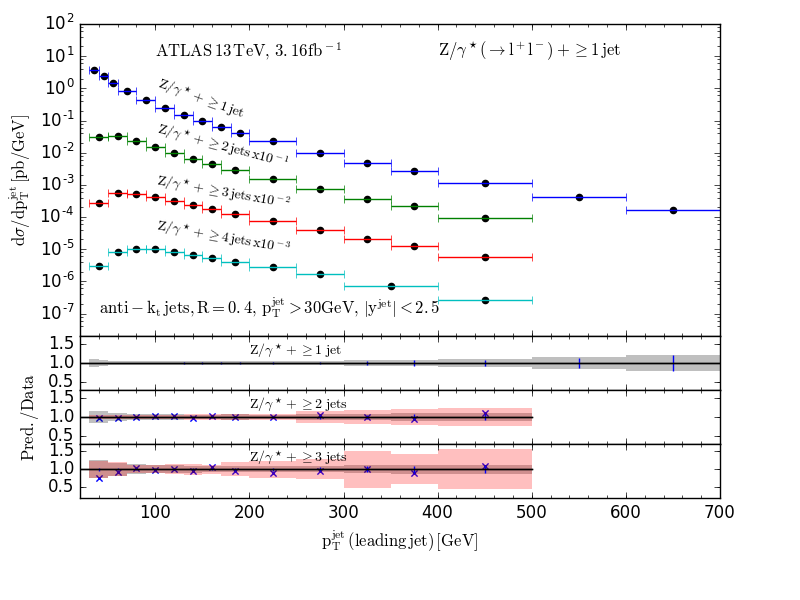
\includegraphics[width=1 \textwidth]{xsection_118CT10.png}

		\caption{Measurements of the cross section as function of the momentum ${p_T}$, with data separated into momentum bins, for inclusive ${Z}$ + 2,3,4 jet events. The data is compared to predictions from BLACKHAT+SHERPA. The blue error bars correspond to the statistical uncertainty and the grey shaded region corresponds to the statistical and systematic uncertainty (including luminosity), which are added in quadrature \cite{HEPD}. The blue crosses show the Prediction/Data ratio. The red region shows the error given by the prediction.}
		\label{xsection}
	\end{center}
\end{figure}
Figure (\ref{xsection}) shows that predictions from BLACKHAT+SHERPA are in agreement with the measured cross section within the systematic uncertainties over the full leading jet ${p_T}$ range. Hence it is appropriate to use predictions from BLACKHAT+SHERPA  from PDF's, for the full range of ${p_T}$, to calculate ${\alpha_s}$. Figure (\ref{xsection}) also shows that the total experimental uncertainty is largely composed of statistical uncertainty for ${p_T = 300-700}$ [GeV], but the statistical uncertainties contribution to the total uncertainty is much smaller for lower values of ${p_T}$. This is because the systematic and luminosity uncertainties are essentially constant for all measurements, as discussed in section (\ref{stats}), but the actual statistical error increases due to there being less scattering events, thus there is less data as the measured cross section has decreased \cite{HEPD}. This is evident in figure (\ref{xsection}). Understanding the origin of the errors is fundamental to a useful extraction of ${\alpha_s}$.
	
\begin{figure} 
	\begin{center}
		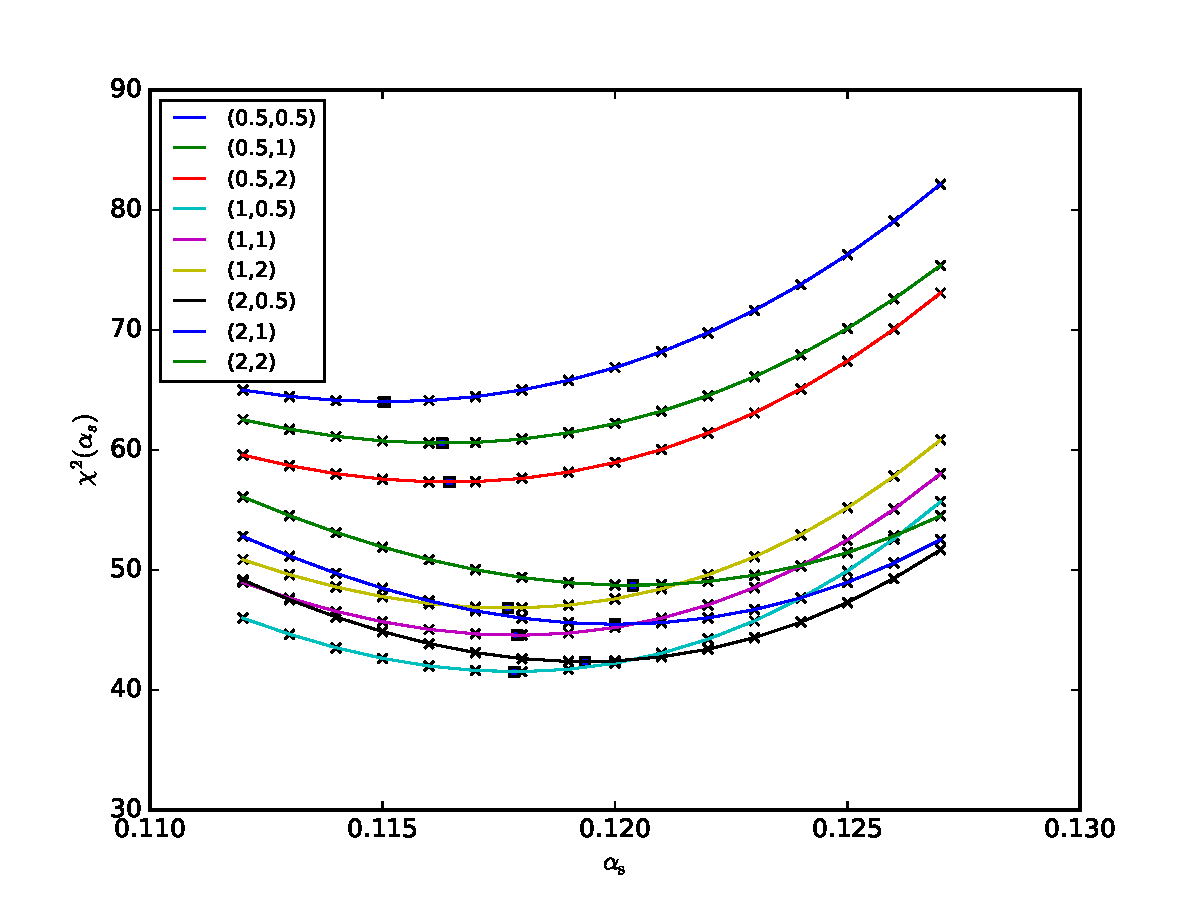
\includegraphics[width=1 \textwidth]{CT10nlo0_curvefit.pdf}
		\caption{A ${\chi ^2}$ test for the CT10nlo PDF at all scale combinations considered. The blue squares represent the minima of each curve and the scale error is found by the envelope of statistics method.}
		\label{CHI}
	\end{center}
\end{figure}


\begin{acknowledgments}
I would like to thank Daniel Ma\^itre, my supervisor. 
\end{acknowledgments}

\begin{thebibliography}{99}
\bibitem{PPB} Particle Date Group, (2017), \url{http://pdg.lbl.gov/2018/reviews/rpp2018-rev-qcd.pdf}, \textit{ Review of Particle Physics: 9. Quantum Chromodynamics}
\bibitem{DMP}M. Johnson and D. Maitre, (2018), \url{https://arxiv.org/pdf/1711.01408.pdf}, \textit{Strong coupling constant extraction from high-multiplicity Z ${^+}$ jets observables.}
\bibitem{HEPD} ATLAS Collaboration (2017), \url{https://www.hepdata.net/record/76542}.
\bibitem{HEPP} ATLAS Collaboration, (2017), \url{https://arxiv.org/pdf/1702.05725.pdf}, \textit{Measurements of Z boson with jets in pp collisions at s=${\sqrt 13}$ TeV.}
\bibitem{PHD} Brooks, Helen, Marguerite (2017), \textit{Multi-jet Phenomenology for Hadron Colliders in the High Energy Limit, Durham theses, Durham University. Available at Durham E-Theses Online: http://etheses.dur.ac.uk/12313/.}
\bibitem{BOOK} M. Peskin and D. Schoeder, (2005), \textit{An Introduction to Quantum Field Theory.}
\bibitem{BLACK} J. Anderson, D. Ma\^itre et al., (2014), \url{https://arxiv.org/abs/1407.1621 [hep-ph]}, \textit{High multiplicity processes with BlackHat and Sherpa.}
\bibitem{MONTE} A. Larkkoski, (2016), \textit{Lecture Notes on Monte Carlo Methods.}


\bibitem{2to3} S. Chatrchyan et al. (CMS), Eur. Phys. J. C73, 2604 (2013), \url{arXiv:1304.7498 [hep-ex]}.
\bibitem{en2en} M. Aaboud et al. (ATLAS), (2017), \url{arXiv:1707.02562 [hep-ex]}.
\bibitem{inc} V. Khachatryan et al. (CMS), Eur. Phys. J. C75, 288 (2015), \url{arXiv:1410.6765 [hep-ex]}.
\bibitem{LEP} R. Frederix, S. Frixione, K. Melnikov, and G. Zanderighi, JHEP 11, 050 (2010), \url{arXiv:1008.5313 [hep-ph]}.
\bibitem{HAD} N. Brambilla, X. Garcia i Tormo, J. Soto, and A. Vairo, Phys. Rev. D75, 074014 (2007), \url{arXiv:hep-ph/0702079 [hep-ph]}.
\bibitem{3jet} V. Khachatryan et al. (CMS), Eur. Phys. J. C75, 186 (2015), \url{arXiv:1412.1633 [hep-ex]}.

\bibitem{GROUP} B. Gutkin, (2016), \textit{Lecture Notes: Group Theory and its applications in physics}
\bibitem{KNL} N. Yoshida, (1982), \url{https://academic.oup.com/ptp/article/67/4/1216/1843144#28365169}, \textit{Progress of Theoretical Physics Supplement No. 77, IV-3. Infrafred Divergences.}
\bibitem{BLACK} J. Campbell, J. Huston, and F. Krauss, The Big Black Book of Quantum Chromodynamics, (2017), Oxford University Press
\bibitem{STAT} D. Yoshioka, (2007), \textit{Statistical Physics.}
\bibitem{LUM} W. Herr and B. Muratori, \url{https://cds.cern.ch/record/941318/files/p361.pdf}, \textit{Concept of Luminosity.}
\bibitem{CT10} H.L. Lai, M. Guzzi, J. Huston, Z. Li, P. M. Nadolsky, et al., \url{Phys.Rev. D82, 074024 (2010), arXiv:1007.2241 [hep-ph]}.
\bibitem{CT14} S. Dulat, T.-J. Hou, J. Gao, M. Guzzi, J. Huston, P. Nadolsky, J. Pumplin, C. Schmidt, D. Stump, and C. P. Yuan, \url{Phys. Rev. D93, 033006 (2016), arXiv:1506.07443 [hep-ph].}
\bibitem{MSTW} A. Martin, W. Stirling, R. Thorne, and G. Watt, Eur. Phys. J. C63, 189 (2009), \url{arXiv:0901.0002 [hep-ph]}.
\bibitem{MMHT1} L. A. Harland-Lang, A. D. Martin, P. Motylinski, and R. S. Thorne, Eur. Phys. J. C75, 204 (2015), \url{arXiv:1412.3989 [hep-ph]}.
\bibitem{MMHT2} L. A. Harland-Lang, A. D. Martin, P. Motylinski, and R. S. Thorne, Eur. Phys. J. C75, 435 (2015), \url{arXiv:1506.05682 [hep-ph]}.
\bibitem{NN23} R. D. Ball et al., Nucl. Phys. B867, 244 (2013), \url{arXiv:1207.1303 [hep-ph]}.
\bibitem{NN30} R. D. Ball et al. (NNPDF), JHEP 04, 040 (2015), \url{arXiv:1410.8849 [hep-ph]}.
\bibitem{LHAPDF} \url{https://lhapdf.hepforge.org/pdfsets}
\bibitem{FAST} D. Britzger, K. Rabbertz, F. Stober, and M. Wobisch (2012) (fastNLO), in Proceedings, \url{arXiv:1208.3641 [hep-ph]}, \textit{20th Inter-national Workshop on Deep-Inelastic Scattering and Related Subjects (DIS 2012) pp.217-221}.
\bibitem{CPDF} S. Alekhin, J. Blumein, and S. Moch, (2012), \url{https://arxiv.org/pdf/1202.2281.pdf}, \textit{Parton distribution functions and benchmark cross sections at NNLO, pg 44.} 
\bibitem{Sca} The CDF Collaboration, (2001), \url{https://www.phys.ufl.edu/~rfield/cdf/chgjet/etaphi.html}, \textit{Charged Jet Evolution under proton-antiproton collisions.}



\end{thebibliography} 


\end{document}

%The Drell-Yan process is interesting as, to leading order in QCD, the cross section required ${\sigma(q\bar{q} \rightarrow l^+l^-)}$ is related to the more simple Quantum Electrodynamic (QED) cross section ${\sigma(e^+e^- \rightarrow q \bar{q})}$. However as quarks are coloured we must average over the colour orientations of the quark and anti-quark, which gives an extra factor of ${\frac{1}{3}}$. This means the cross-section is given by: \begin{equation} \label{cross} \sigma(q_f\bar{q_f} \xrightarrow{Z} l^+l^-) = \frac{1}{3}Q_f^2 \dfrac{4\pi\alpha^2}{3\hat{s}}, \end{equation} where ${f}$ subscript represents the quark flavours, ${Q_f}$ represents the electric charge of that quark and ${\hat{s}}$ represents the centre of mass energy. Here ${\alpha = \frac{1}{137}}$ and is denoted the fine structure constant. Equation (\ref{cross}) assumes that the centre of mass energy is high enough to ignore the quark masses \cite{BOOK}.